\documentclass[border=8pt]{standalone}
\usepackage[T1]{fontenc}
\usepackage{amsmath,amssymb}
\usepackage{tikz}
\usetikzlibrary{arrows.meta,decorations.pathreplacing,calc}
\renewcommand{\familydefault}{\sfdefault}

\definecolor{kthblue}{HTML}{004791}
\definecolor{kthlight}{HTML}{DEF0FC}
\definecolor{kthorange}{HTML}{E37222}
\definecolor{kthdark}{HTML}{000061}
\definecolor{kthmid}{HTML}{6298D2}
\definecolor{kthgreen}{HTML}{3F8F4F}

\newcommand{\bV}{\mathbf{V}}
\newcommand{\bU}{\mathbf{U}}
\newcommand{\bH}{\mathbf{H}}
\newcommand{\bn}{\mathbf{n}}
\newcommand{\RF}{\mathrm{RF}}

\begin{document}
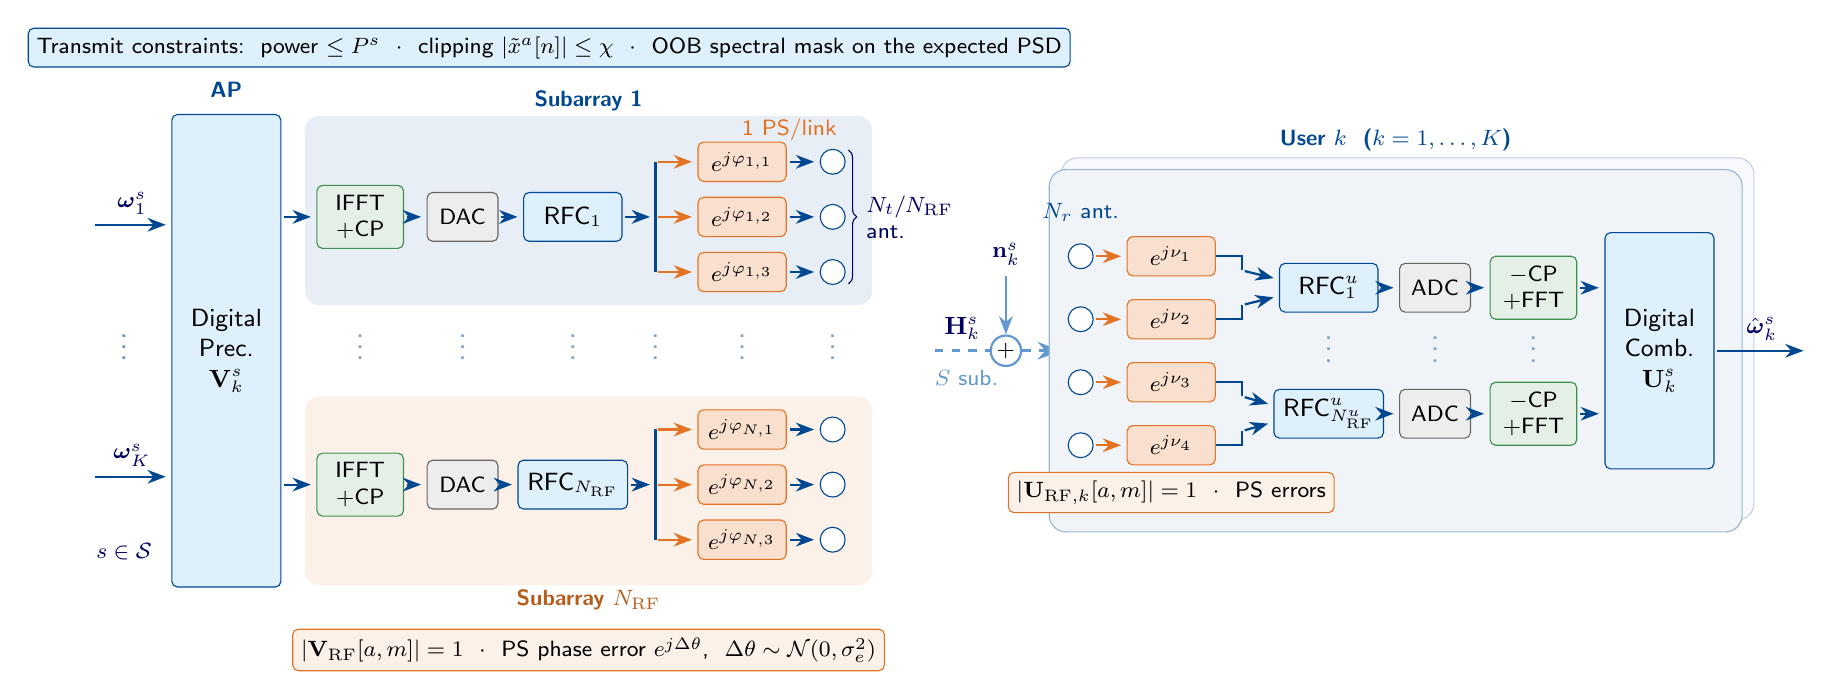
\begin{tikzpicture}[
    font=\small,
    x=1cm,y=1cm,
    rfc/.style={draw=kthblue,fill=kthlight,rounded corners=2pt,
        minimum width=1.25cm,minimum height=0.62cm,align=center,font=\small},
    ofdm/.style={draw=kthgreen,fill=kthgreen!14,rounded corners=2pt,
        minimum width=1.10cm,minimum height=0.80cm,align=center,font=\footnotesize,inner sep=1pt},
    conv/.style={draw=black!60,fill=black!7,rounded corners=2pt,
        minimum width=0.90cm,minimum height=0.62cm,align=center,font=\footnotesize},
    psh/.style={draw=kthorange,fill=kthorange!22,rounded corners=2pt,
        minimum width=1.12cm,minimum height=0.50cm,align=center,font=\footnotesize,inner sep=1pt},
    ant/.style={draw=kthblue,fill=white,circle,inner sep=0pt,minimum size=9pt},
    arr/.style={->,>=Stealth,thick,kthblue,shorten <=1pt,shorten >=2pt},
    note/.style={font=\footnotesize,draw=kthorange,fill=kthorange!10,rounded corners=2pt,
        inner sep=3pt,align=center},
    cnote/.style={font=\footnotesize,draw=kthblue,fill=kthlight,rounded corners=2pt,
        inner sep=3pt,align=center},
    ]

    %---------------------------------------------------------
    % TRANSMITTER (AP)
    %---------------------------------------------------------
    \node[rfc, minimum height=6.0cm, minimum width=1.35cm, text width=1.15cm]
        (dig) at (0.75,0){Digital\\Prec.\\$\bV_k^s$};
    \node[font=\footnotesize\bfseries,kthblue,above=0.08cm] at (dig.north){AP};

    % data streams into the digital precoder
    \draw[arr](-0.95,1.60)--node[above,font=\footnotesize,kthdark]{$\boldsymbol{\omega}_1^s$}(dig.west|-0,1.60);
    \draw[arr](-0.95,-1.60)--node[above,font=\footnotesize,kthdark]{$\boldsymbol{\omega}_K^s$}(dig.west|-0,-1.60);
    \node[kthblue!60,font=\large] at (-0.55,0.15){$\vdots$};
    \node[font=\footnotesize,kthdark,align=center] at (-0.55,-2.55){$s\in\mathcal{S}$};

    % constraints on the transmitted waveform
    \node[cnote] at (4.85,3.85)
        {Transmit constraints:\ \ power $\le P^s$ \ $\cdot$ \ clipping $|\tilde{x}^a[n]|\le\chi$
         \ $\cdot$ \ OOB spectral mask on the expected PSD};

    % ---- Subarray 1 ----
    \fill[kthblue!9,rounded corners=5pt] (1.75,0.58) rectangle (8.95,2.98);
    \node[font=\footnotesize\bfseries,kthblue] at (5.35,3.17){Subarray 1};

    \node[ofdm](ifft1) at (2.45,1.70){IFFT\\+CP};
    \node[conv](dac1)  at (3.75,1.70){DAC};
    \node[rfc](rfc1)   at (5.15,1.70){RFC$_1$};
    \draw[arr](dig.east|-ifft1)--(ifft1.west);
    \draw[arr](ifft1.east)--(dac1.west);
    \draw[arr](dac1.east)--(rfc1.west);

    \draw[arr](rfc1.east)--(6.20,1.70);
    \draw[kthblue,thick](6.20,1.00)--(6.20,2.40);

    \node[psh](psa) at (7.30,2.40){$e^{j\varphi_{1,1}}$};
    \node[ant](anta) at (8.45,2.40){};
    \draw[arr,kthorange](6.20,2.40)--(psa.west);
    \draw[arr](psa.east)--(anta.west);

    \node[psh](psb) at (7.30,1.70){$e^{j\varphi_{1,2}}$};
    \node[ant](antb) at (8.45,1.70){};
    \draw[arr,kthorange](6.20,1.70)--(psb.west);
    \draw[arr](psb.east)--(antb.west);

    \node[psh](psc) at (7.30,1.00){$e^{j\varphi_{1,3}}$};
    \node[ant](antc) at (8.45,1.00){};
    \draw[arr,kthorange](6.20,1.00)--(psc.west);
    \draw[arr](psc.east)--(antc.west);

    \draw[decorate,decoration={brace,amplitude=3pt},kthdark]
        (8.65,2.55)--(8.65,0.85)
        node[midway,right=3pt,kthdark,font=\footnotesize,align=left]{$N_t/N_\RF$\\ant.};
    \node[font=\footnotesize,kthorange] at (7.90,2.80){1 PS/link};

    \foreach \x in {2.45,3.75,5.15,6.20,7.30,8.45}{
        \node[kthblue!50,font=\large] at (\x,0.15){$\vdots$};
    }

    % ---- Subarray N_RF ----
    \fill[kthorange!10,rounded corners=5pt] (1.75,-2.98) rectangle (8.95,-0.58);
    \node[font=\footnotesize\bfseries,kthorange!80!black] at (5.35,-3.17){Subarray $N_\RF$};

    \node[ofdm](ifftN) at (2.45,-1.70){IFFT\\+CP};
    \node[conv](dacN)  at (3.75,-1.70){DAC};
    \node[rfc](rfcN)   at (5.15,-1.70){RFC$_{N_\RF}$};
    \draw[arr](dig.east|-ifftN)--(ifftN.west);
    \draw[arr](ifftN.east)--(dacN.west);
    \draw[arr](dacN.east)--(rfcN.west);

    \draw[arr](rfcN.east)--(6.20,-1.70);
    \draw[kthblue,thick](6.20,-2.40)--(6.20,-1.00);

    \node[psh](psd) at (7.30,-1.00){$e^{j\varphi_{N,1}}$};
    \node[ant](antd) at (8.45,-1.00){};
    \draw[arr,kthorange](6.20,-1.00)--(psd.west);
    \draw[arr](psd.east)--(antd.west);

    \node[psh](pse) at (7.30,-1.70){$e^{j\varphi_{N,2}}$};
    \node[ant](ante) at (8.45,-1.70){};
    \draw[arr,kthorange](6.20,-1.70)--(pse.west);
    \draw[arr](pse.east)--(ante.west);

    \node[psh](psf) at (7.30,-2.40){$e^{j\varphi_{N,3}}$};
    \node[ant](antf) at (8.45,-2.40){};
    \draw[arr,kthorange](6.20,-2.40)--(psf.west);
    \draw[arr](psf.east)--(antf.west);

    \node[note] at (5.35,-3.80)
        {$|\bV_\RF[a,m]|=1$ \ $\cdot$ \ PS phase error $e^{j\Delta\theta}$, \ $\Delta\theta\sim\mathcal{N}(0,\sigma_e^2)$};

    \begin{scope}[xshift=0.3cm]
    %---------------------------------------------------------
    % CHANNEL + NOISE
    %---------------------------------------------------------
    \node[draw=kthmid,thick,circle,inner sep=0pt,minimum size=11pt,font=\footnotesize] (sum) at (10.35,0){$+$};
    \draw[kthmid,dashed,very thick](9.45,0)--node[above,font=\small,kthdark]{$\bH_k^s$}(sum.west);
    \node[font=\footnotesize,kthmid,below=0.12cm] at (9.85,0){$S$ sub.};
    \draw[->,>=Stealth,thick,kthmid](10.35,0.95)node[above,font=\footnotesize,kthdark]{$\bn_k^s$}--(sum.north);
    \draw[->,>=Stealth,kthmid,dashed,very thick](sum.east)--(11.05,0);

    %---------------------------------------------------------
    % USER k (one of K)
    %---------------------------------------------------------
    \fill[kthblue!3,rounded corners=6pt,draw=kthblue!25] (11.05,-2.15) rectangle (19.85,2.45);
    \fill[kthblue!6,rounded corners=6pt,draw=kthblue!40] (10.90,-2.30) rectangle (19.70,2.30);
    \node[font=\footnotesize\bfseries,kthblue] at (15.30,2.68){User $k$ \ ($k=1,\dots,K$)};

    \node[ant](rxa1) at (11.30, 1.20){};
    \node[ant](rxa2) at (11.30, 0.40){};
    \node[ant](rxa3) at (11.30,-0.40){};
    \node[ant](rxa4) at (11.30,-1.20){};
    \node[font=\footnotesize,kthblue,above=2pt] at (11.30,1.45){$N_r$ ant.};

    \node[psh](psr1) at (12.45, 1.20){$e^{j\nu_1}$};
    \node[psh](psr2) at (12.45, 0.40){$e^{j\nu_2}$};
    \node[psh](psr3) at (12.45,-0.40){$e^{j\nu_3}$};
    \node[psh](psr4) at (12.45,-1.20){$e^{j\nu_4}$};

    \node[rfc](urfc1) at (14.45, 0.80){RFC$_1^u$};
    \node[rfc](urfcN) at (14.45,-0.80){RFC$_{N_\RF^u}^u$};
    \node[conv](adc1) at (15.80, 0.80){ADC};
    \node[conv](adcN) at (15.80,-0.80){ADC};
    \node[ofdm](fft1) at (17.05, 0.80){$-$CP\\+FFT};
    \node[ofdm](fftN) at (17.05,-0.80){$-$CP\\+FFT};
    \foreach \x in {14.45,15.80,17.05}{
        \node[kthblue!50,font=\large] at (\x,0.12){$\vdots$};
    }

    \node[rfc,minimum height=3.0cm,minimum width=1.35cm,text width=1.15cm]
        (udig) at (18.65,0){Digital\\Comb.\\$\bU_k^s$};

    \draw[arr,kthorange](rxa1.east)--(psr1.west);
    \draw[arr,kthorange](rxa2.east)--(psr2.west);
    \draw[arr,kthorange](rxa3.east)--(psr3.west);
    \draw[arr,kthorange](rxa4.east)--(psr4.west);

    \draw[kthblue,thick] (psr1.east)--(13.35,1.20)--(13.35,1.02);
    \draw[arr]           (13.35,1.02)--([yshift=3pt]urfc1.west);
    \draw[kthblue,thick] (psr2.east)--(13.35,0.40)--(13.35,0.58);
    \draw[arr]           (13.35,0.58)--([yshift=-3pt]urfc1.west);
    \draw[kthblue,thick] (psr3.east)--(13.35,-0.40)--(13.35,-0.58);
    \draw[arr]           (13.35,-0.58)--([yshift=3pt]urfcN.west);
    \draw[kthblue,thick] (psr4.east)--(13.35,-1.20)--(13.35,-1.02);
    \draw[arr]           (13.35,-1.02)--([yshift=-3pt]urfcN.west);

    \draw[arr](urfc1.east)--(adc1.west);
    \draw[arr](urfcN.east)--(adcN.west);
    \draw[arr](adc1.east)--(fft1.west);
    \draw[arr](adcN.east)--(fftN.west);
    \draw[arr](fft1.east)--(udig.west|-fft1);
    \draw[arr](fftN.east)--(udig.west|-fftN);

    \draw[arr](udig.east)--node[above,font=\footnotesize,kthdark]{$\hat{\boldsymbol{\omega}}_k^s$}(20.55,0);

    \node[note] at (12.45,-1.80){$|\bU_{\RF,k}[a,m]|=1$ \ $\cdot$ \ PS errors};

    \end{scope}
\end{tikzpicture}
\end{document}
